A continuación se detallará la vista completa del módulo \textit{landportal\_uris}.  Tal y como se ha explicado anteriormente en la vista del gestor de contenidos, se omitirá la presentación de las vistas del resto de módulos debido su baja complejidad, ya que estarán formados por un único fichero donde se implementa el \textit{hook} correspondiente.

\subsubsection{Diagrama de componentes}
La figura \ref{fig:diagrama_componentes_landportal_uris} muestra el diagrama de los componentes que forman parte del módulo ``\textit{landportal\_uris}''.
\begin{landscape}
	\begin{figure}[ht]
		\centering
		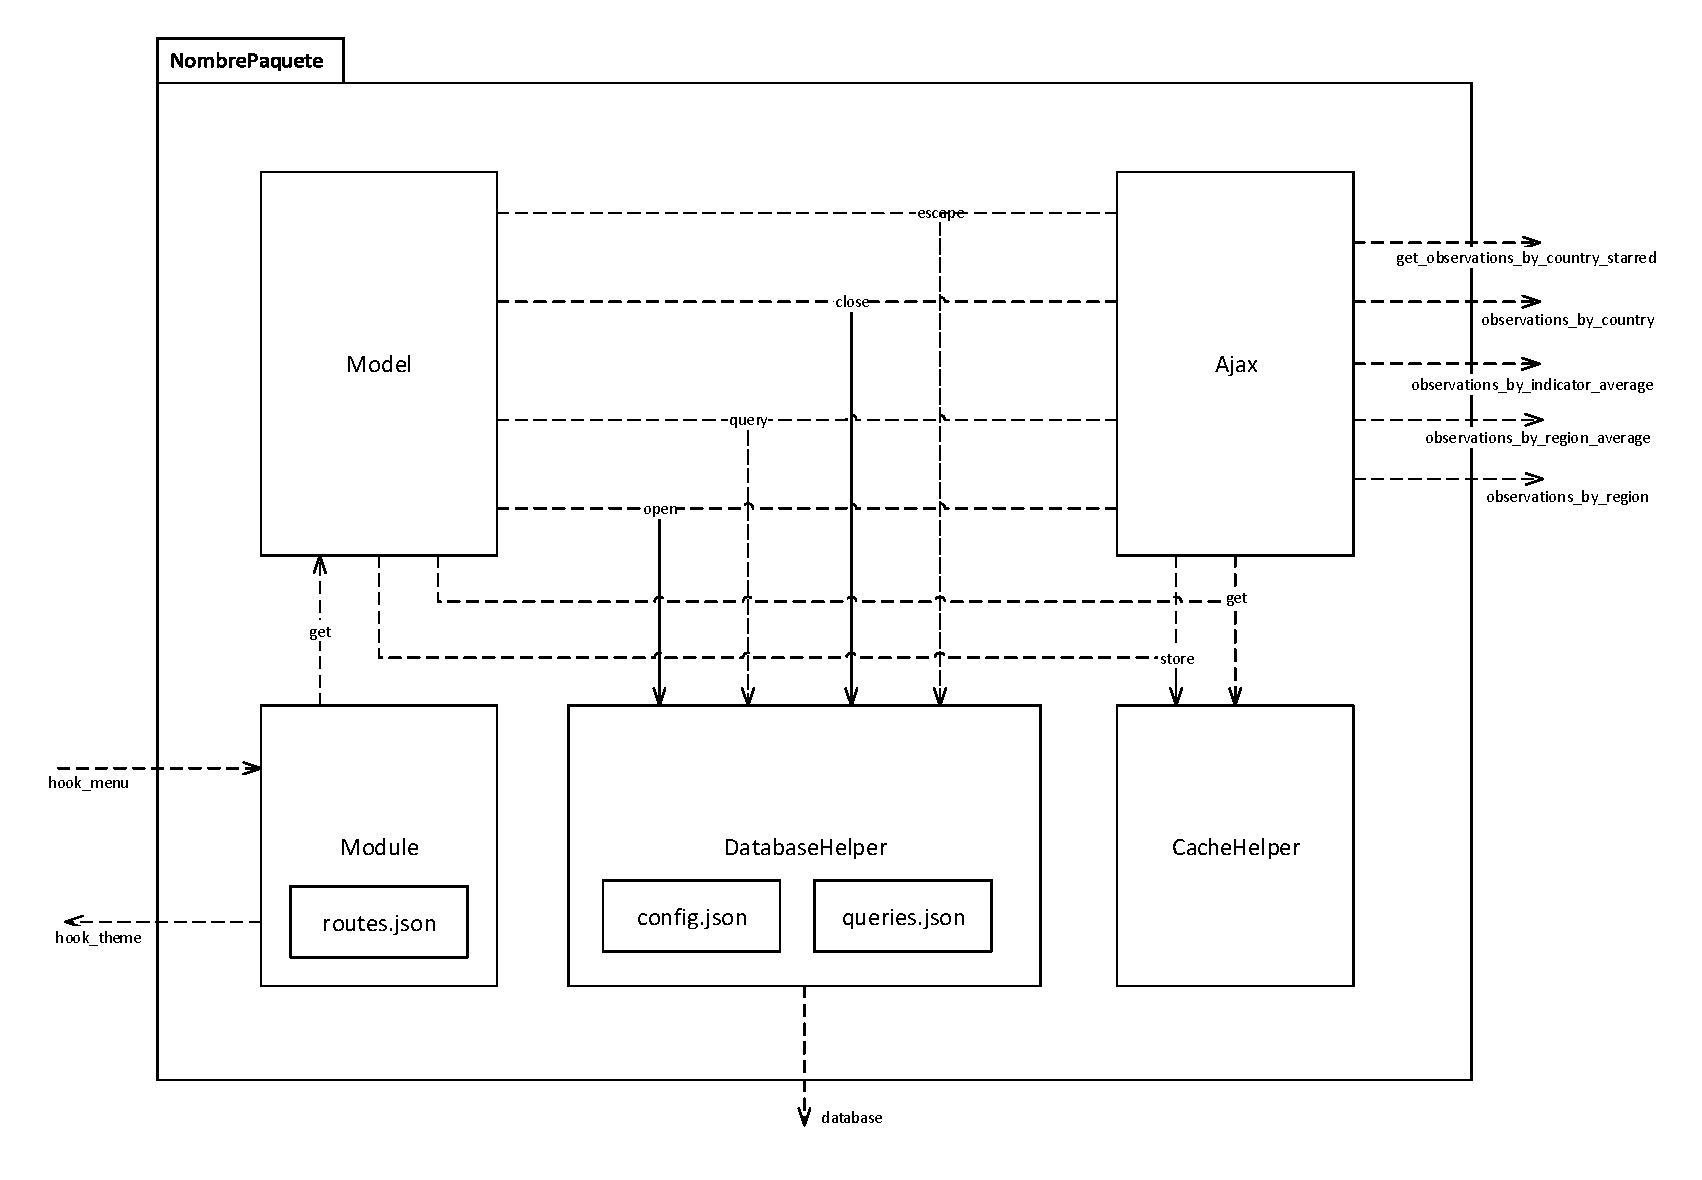
\includegraphics[height=\textwidth]{arquitectura/landportal_uris_view}
		\caption{Diagrama de componentes del módulo ``\textit{landportal\_uris}''}
		\label{fig:diagrama_componentes_landportal_uris}
	\end{figure}
\end{landscape}


\subsubsection{Descripción de los componentes}
Se describirán ahora los distintos componentes que forman parte del módulo ``\textit{landportal\_uris}''.  La organización de dichos componentes puede verse en la figura \ref{fig:diagrama_componentes_landportal_uris}
\begin{description}
	\item[Module]  Contiene la implementación del \textit{hook} que el gestor de contenidos utilizará para llamar a éste módulo.  Es el principal punto de entrada al módulo.  Incluye un fichero donde se declararán las rutas y las vistas que estarán disponibles.
	\item[DatabaseHelper]  Funciona como una capa de abstracción sobre la base de datos.  Ofrece una serie de métodos que serán utilizados por el resto de componentes que necesiten acceder a la base de datos.  Incluye un fichero que configura la información de conexión a la base de datos y otro que incluye las consultas disponibles.
	\item[CacheHelper]  Permite el cacheo de datos con el fin de agilizar la consulta y procesado de grandes cantidades de datos.  Ofrece una serie de métodos que serán utilizados por el resto de componentes que necesiten acceder al caché.
	\item[Ajax]  Implementa el framewok que da soporte a la creación de visualizaciones.  Expone varias interfaces que serán utilizadas por las visualizaciones para obtener los datos que posteriormente presentarán a los usuarios.
	\item[Model]  Devuelve los datos necesarios para presentar las diferentes vistas del sistema.  Los modelos se invocarán utilizando un convenio de nombres en función de la vista a la que pertencezcan.
\end{description}

\subsubsection{Relación entre los componentes}
El módulo lee la configuración de rutas desde el fichero ``\textit{routes.json}''.  Con cada petición recibida desde el núcleo del gestor de contenidos se buscará el modelo correspondiente a la vista mediante un convenio de nombres y se invocará su funcionalidad.  Posteriormente se invocará al tema para que renderice la vista adecuada.

Los modelos cargarán los datos necesarios para la renderización de la vista a través de diferentes consultas a la base de datos.  
El framework de soporte a visualizaciones funcionará de forma similar a los modelos, realizando consultas a la base de datos para obtener los datos necesarios.

En ambos casos, para agilizar la consulta y el procesamiento de los datos, los resultados se cachearán antes de ser devueltos, de forma que las posteriores peticiones accedan directamente a la información del caché.


\subsubsection{Interfaces y puertos}
A continuación se detallarán las interfaces y puertos de los componentes que forman parte del módulo ``\textit{landportal\_uris}''.

\paragraph{LandPortal URIs} \hfill \\
La tabla \ref{interfaces_landportal_uris_landportal_uris} muestra el detalle de las interfaces del módulo ``\textit{LandPortal URIs}''.  

\begin{longtable}[c]{|p{25mm}|p{20mm}|p{30mm}|p{60mm}|}
	\caption{Vista del módulo \textit{LandPortal URIs}- interfaces del módulo \textit{LandPortal URIs}. \label{interfaces_landportal_uris_landportal_uris}}\\
	%Cabecera en la primera pagina
		\hline
			Interfaz & Tipo & Tecnología & Propiedades\\
		\hline
		\hline
	\endfirsthead
	%Cabecera en el resto de páginas
		\hline
		\multicolumn{4}{|c|}{Continuación de la tabla \ref{interfaces_landportal_uris_landportal_uris}}\\
		\hline
			Interfaz & Tipo & Tecnología & Propiedades\\
		\hline
		\hline
	\endhead
	%Tabla
	\hline
	\endfoot
		\textbf{hook menu} & Proveída & Llamada a método & Invocado por el gestor de contenidos durante la definición de las rutas que tendrán las vistas del portal \\
		\hline
		\textbf{hook theme} & Requerida & Llamada a método & Pide al tema que renderice una determinada plantilla para una vista \\
		\hline
		\textbf{get observations by country starred} & Proveída & API Web & Devuelve todas las observaciones referentes a un determinado país para los indicadores favoritos \\
		\hline
		\textbf{observations by country} & Proveída & API Web & Devuelve todas las observaciones referentes a un determinado país sin tener en cuenta el indicador \\
		\hline
		\textbf{get observations by indicator average} & Proveída & API Web & Devuelve el valor medio de todas las observaciones para un determinado indicador \\
		\hline
		\textbf{get observations by region average} & Proveída & API Web & Devuelve el valor medio de todas las observaciones referente a una determinada región sin tener en cuenta el indicador \\
		\hline
		\textbf{observations by region} & Proveída & API Web & Devuelve todas las observaciones referentes a una determinada región sin tener en cuenta el indicador \\
		\hline
		\textbf{database} & Requerida & Conexión a base de datos & Obtiene información de la base de datos \\
	\hline
	\hline
\end{longtable}

\paragraph{Module} \hfill \\
La tabla \ref{interfaces_landportal_uris_module} muestra el detalle de las interfaces del componente ``\textit{module}''.  

\begin{longtable}[c]{|p{25mm}|p{20mm}|p{30mm}|p{60mm}|}
	\caption{Vista del módulo \textit{LandPortal URIs}- interfaces del componente ``\textit{module}''. \label{interfaces_landportal_uris_module}}\\
	%Cabecera en la primera pagina
		\hline
			Interfaz & Tipo & Tecnología & Propiedades\\
		\hline
		\hline
	\endfirsthead
	%Cabecera en el resto de páginas
		\hline
		\multicolumn{4}{|c|}{Continuación de la tabla \ref{interfaces_landportal_uris_module}}\\
		\hline
			Interfaz & Tipo & Tecnología & Propiedades\\
		\hline
		\hline
	\endhead
	%Tabla
	\hline
	\endfoot
		\textbf{hook menu} & Puerto de entrada & Llamada a método & Invocado por el gestor de contenidos durante la definición de las rutas que tendrán las vistas del portal \\
		\hline
		\textbf{hook theme} & Requerida & Llamada a método & Pide al tema que renderice una determinada plantilla para una vista \\
		\hline
		\textbf{get} & Puerto de salida & Llamada a método & Pide a un modelo los datos necesarios para que posteriormente el tema renderice la vista \\
		\hline
	\hline
	\hline
\end{longtable}


\paragraph{DatabaseHelper} \hfill \\
La tabla \ref{interfaces_landportal_uris_databasehelper} muestra el detalle de las interfaces del componente ``\textit{DatabaseHelper}''.  

\begin{longtable}[c]{|p{25mm}|p{20mm}|p{30mm}|p{60mm}|}
	\caption{Vista del módulo \textit{LandPortal URIs}- interfaces del componente ``\textit{DatabaseHelper}''. \label{interfaces_landportal_uris_databasehelper}}\\
	%Cabecera en la primera pagina
		\hline
			Interfaz & Tipo & Tecnología & Propiedades\\
		\hline
		\hline
	\endfirsthead
	%Cabecera en el resto de páginas
		\hline
		\multicolumn{4}{|c|}{Continuación de la tabla \ref{interfaces_landportal_uris_databasehelper}}\\
		\hline
			Interfaz & Tipo & Tecnología & Propiedades\\
		\hline
		\hline
	\endhead
	%Tabla
	\hline
	\endfoot
		\textbf{open} & Puerto de entrada & Llamada a método & Abre una conexión con la base de datos \\
		\hline
		\textbf{query} & Puerto de entrada & Llamada a método & Realiza una consulta a la base de datos y devuelve su resultado \\
		\hline
		\textbf{close} & Puerto de entrada & Llamada a método & Cierra una conexión con la base de datos \\
		\hline
		\textbf{escape} & Puerto de entrada & Llamada a método & Escapa los parámetros de una consulta antes de enviarla a la base de datos\footnote{El escapado de argumentos es un procedimiento necesario para evitar ataques del tipo \textit{SQLInjection} cuando no se utilizan \textit{PreparedStatements}.  Para más información al respecto véase \url{http://www.php.net/manual/en/mysqli.real-escape-string.php}} \\
		\hline
		\textbf{database} & Puerto de salida & Conexión a base de datos & Obtiene información de la base de datos \\
	\hline
	\hline
\end{longtable}


\paragraph{CacheHelper} \hfill \\
La tabla \ref{interfaces_landportal_uris_cachehelper} muestra el detalle de las interfaces del componente ``\textit{CacheHelper}''.  

\begin{longtable}[c]{|p{25mm}|p{20mm}|p{30mm}|p{60mm}|}
	\caption{Vista del módulo \textit{LandPortal URIs}- interfaces del componente ``\textit{CacheHelper}''. \label{interfaces_landportal_uris_cachehelper}}\\
	%Cabecera en la primera pagina
		\hline
			Interfaz & Tipo & Tecnología & Propiedades\\
		\hline
		\hline
	\endfirsthead
	%Cabecera en el resto de páginas
		\hline
		\multicolumn{4}{|c|}{Continuación de la tabla \ref{interfaces_landportal_uris_cachehelper}}\\
		\hline
			Interfaz & Tipo & Tecnología & Propiedades\\
		\hline
		\hline
	\endhead
	%Tabla
	\hline
	\endfoot
		\textbf{get} & Puerto de entrada & Llamada a método & Obtiene el elemento almacenado en el caché bajo una determinada clave \\
		\hline
		\textbf{store} & Puerto de entrada & Llamada a método & Almacena un elemento en el caché utilizando una determinada clave que posteriormente podrá ser utilizada para recuperarlo \\
		\hline
	\hline
	\hline
\end{longtable}

\paragraph{Model} \hfill \\
La tabla \ref{interfaces_landportal_model} muestra el detalle de las interfaces comunes a todos los modelos.  

\begin{longtable}[c]{|p{25mm}|p{20mm}|p{30mm}|p{60mm}|}
	\caption{Vista del módulo \textit{LandPortal URIs}- interfaces del componente ``\textit{Model}''. \label{interfaces_landportal_model}}\\
	%Cabecera en la primera pagina
		\hline
			Interfaz & Tipo & Tecnología & Propiedades\\
		\hline
		\hline
	\endfirsthead
	%Cabecera en el resto de páginas
		\hline
		\multicolumn{4}{|c|}{Continuación de la tabla \ref{interfaces_landportal_model}}\\
		\hline
			Interfaz & Tipo & Tecnología & Propiedades\\
		\hline
		\hline
	\endhead
	%Tabla
	\hline
	\endfoot
		\textbf{open} & Puerto de salida & Llamada a método & Abre una conexión con la base de datos \\
		\hline
		\textbf{query} & Puerto de salida & Llamada a método & Realiza una consulta a la base de datos y devuelve su resultado \\
		\hline
		\textbf{close} & Puerto de salida & Llamada a método & Cierra una conexión con la base de datos \\
		\hline
		\textbf{escape} & Puerto de salida & Llamada a método & Escapa los parámetros de una consulta antes de enviarla a la base de datos \\
		\hline
		\textbf{get} & Puerto de entrada & Llamada a método & Devuelve la información necesaria para que el tema renderice la vista correspondiente \\
		\hline
		\textbf{get (CacheHelper)} & Puerto de salida & Llamada a método & Obtiene el elemento almacenado en el caché bajo una determinada clave \\
		\hline
		\textbf{store} & Puerto de salida & Llamada a método & Almacena un elemento en el caché utilizando una determinada clave que posteriormente podrá ser utilizada para recuperarlo \\
	\hline
	\hline
\end{longtable}


\paragraph{Ajax} \hfill \\
La tabla \ref{interfaces_landportal_ajax} muestra el detalle de las interfaces pertenecientes al framework de soporte a las visualizaciones.  

\begin{longtable}[c]{|p{25mm}|p{20mm}|p{30mm}|p{60mm}|}
	\caption{Vista del módulo \textit{LandPortal URIs}- interfaces del componente ``\textit{Ajax}''. \label{interfaces_landportal_ajax}}\\
	%Cabecera en la primera pagina
		\hline
			Interfaz & Tipo & Tecnología & Propiedades\\
		\hline
		\hline
	\endfirsthead
	%Cabecera en el resto de páginas
		\hline
		\multicolumn{4}{|c|}{Continuación de la tabla \ref{interfaces_landportal_ajax}}\\
		\hline
			Interfaz & Tipo & Tecnología & Propiedades\\
		\hline
		\hline
	\endhead
	%Tabla
	\hline
	\endfoot
		\textbf{open} & Puerto de salida & Llamada a método & Abre una conexión con la base de datos \\
		\hline
		\textbf{query} & Puerto de salida & Llamada a método & Realiza una consulta a la base de datos y devuelve su resultado \\
		\hline
		\textbf{close} & Puerto de salida & Llamada a método & Cierra una conexión con la base de datos \\
		\hline
		\textbf{escape} & Puerto de salida & Llamada a método & Escapa los parámetros de una consulta antes de enviarla a la base de datos \\
		\hline
		\textbf{get (CacheHelper)} & Puerto de salida & Llamada a método & Obtiene el elemento almacenado en el caché bajo una determinada clave \\
		\hline
		\textbf{store} & Puerto de salida & Llamada a método & Almacena un elemento en el caché utilizando una determinada clave que posteriormente podrá ser utilizada para recuperarlo \\
		\hline
		\textbf{get observations by country starred} & Puerto de salida & API Web & Devuelve todas las observaciones referentes a un determinado país para los indicadores favoritos \\
		\hline
		\textbf{observations by country} & Puerto de salida & API Web & Devuelve todas las observaciones referentes a un determinado país sin tener en cuenta el indicador \\
		\hline
		\textbf{get observations by indicator average} & Puerto de salida & API Web & Devuelve el valor medio de todas las observaciones para un determinado indicador \\
		\hline
		\textbf{get observations by region average} & Puerto de salida & API Web & Devuelve el valor medio de todas las observaciones referente a una determinada región sin tener en cuenta el indicador \\
		\hline
		\textbf{observations by region} & Puerto de salida & API Web & Devuelve todas las observaciones referentes a una determinada región sin tener en cuenta el indicador \\
		\hline
	\hline
	\hline
\end{longtable}